\chapter{Simulation Results}
\label{chapter:simulation-results}

In the simulation, in total 2000 different agent types (different triples of the type [$\mu$, $\sigma$, $\alpha$]) are present in the population. Every single of these 2000 agents got to communicate with every other agent. This makes in total $2000 \cdot 2000 = 4000000$ EU computations between different types of agents. In the following section, the expected utility data will be presented, described and interpreted.

\section{EU results}
\label{sec:eu-results}
Because of the amount of data points that are to be displayed, I chose a heatmap visualization for the EU results. Different types/parameters of interest are mapped on rows and columns of a two-dimensional matrix. Each cell in this matrix contains an EU score of $type_i$ vs. $type_j$.
The cells are colored depending on the EU score, with blue indicating low values, white for medium values and red indicating high values. An exact color-value-mapping can be found on the top left side of each plot.
To visually inspect the main effects of the three parameters that define an agent type ($\mu$, $\sigma$, $\alpha$) on the EU score, I marginalized out each parameter respectively. In Figure \ref{figure:alpha_marg}, a heatmap visualization is presented for the effect of the parameter $\alpha$.
\begin{figure}[h]
 \centering
 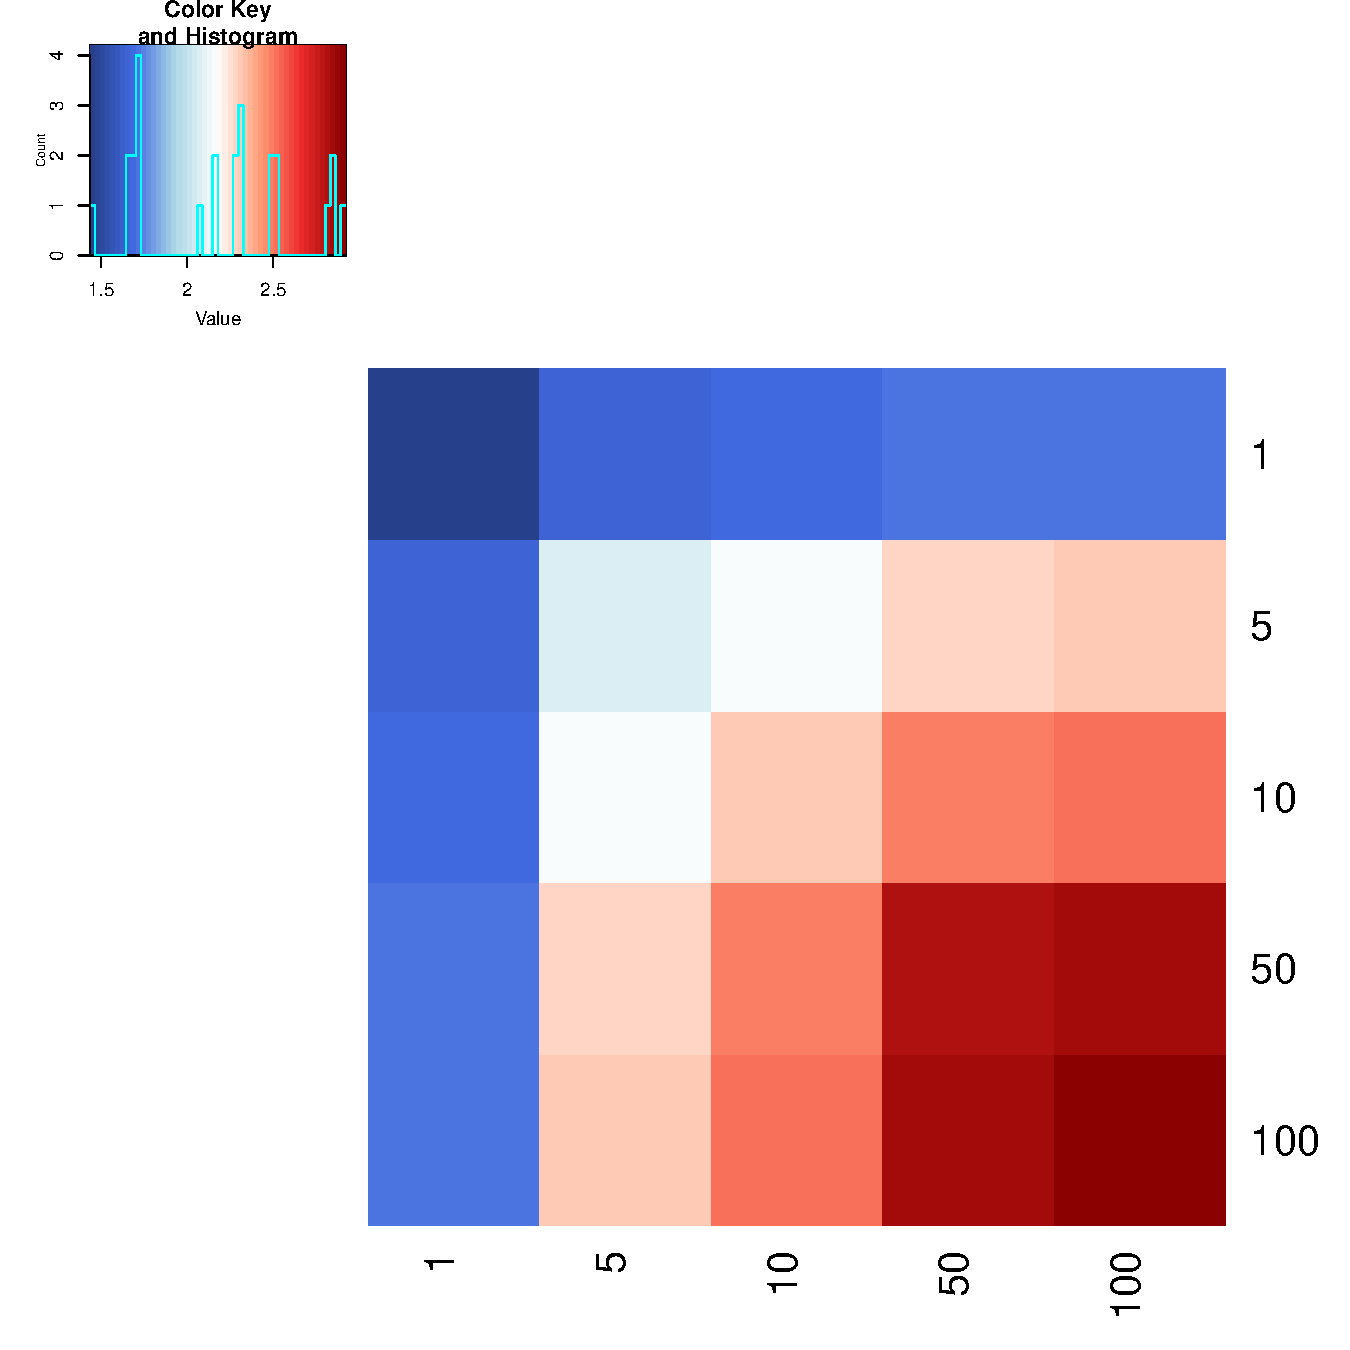
\includegraphics[width=0.7\textwidth]{alpha_marg.pdf}
 \caption{Effect of type parameter $\alpha$ on EU scores.}
 \label{figure:alpha_marg}
\end{figure}
On the x and y axis the possible alpha values are listed (1, 5, 10, 50, 100), in increasing order from left to right and top to bottom. One cell is an EU score of $type_i$ vs $type_j$. E.g. the top right cell contains the mean EU score that is obtained when a type with $\alpha=1$ plays with a type with $\alpha=100$ (that is the mean EU value of all types that have any possible $\mu$ and $\sigma$ values combined with this alpha).\\

The top row and left column (where $\alpha = 1$ on sender- and receiver side) contain low EU scores, this means that the overall success of irrational agents is rather low. In contrast, when looking at the bottom right cell, which contains the EU value of two maximally rational agents, the overall maximum score is obtained.
In conclusion, the EU scores increase with increasing alpha (top left cell: $\alpha=1$ vs. $\alpha=1$, bottom right cell: $\alpha=100$ vs. $\alpha=100$). This is because informative message choices on the speaker side and pragmatic inference methods on the listener side result in higher communicative success than more random choices. 
\begin{figure}[h]
 \centering
 \includegraphics[width=0.7\textwidth]{mean_marg.pdf}
 \caption{Effect of type parameter $\mu$ on EU scores.}
 \label{figure:mean_marg}
\end{figure}
Figure \ref{figure:mean_marg} shows a heatmap plot for the effect of the $Pr(\theta)$ distribution parameter $\mu$. 
Again, all possible $\mu$'s (0, 0.1, 0.2, ..., 1.9) are listed on the axes in an increasing order from left to right and top to bottom. Again, one cell is a mean EU score that is obtained when types with $\mu_i$ play with types with $\mu_j$.
While low values like 0 or 0.1 generally lead to low EU scores (top row and left column), the highest scores can be obtained when both agents have a belief about the threshold with a $\mu$ between 0.5 and 0.9 (indicated by the dark red spot in the middle). This is because very weak interpretations, i.e. low threshold values, will mean that \textit{tall} is true for almost all world states, which is not informative. A very high threshold value is dispreferred because it restricts \textit{tall} to be true for just a few world states that are very likely to be false \textit{a priori}. It seems natural that rather medium values for $\mu_{\theta}$, that capture the meaning of \textit{tall} loosely as \textit{taller than average}, lead to the highest EU scores.\\

The effect of $\sigma$ is presented in Fig.\ref{figure:sigma_marg}. The ordering of possible $\sigma$'s (0.001, 0.1, 0.2, ... 1.9) is similar to the other two plots, increasing from top to bottom and left to right. The effect of $\sigma$ is particularly interesting, as it reflects the effect of "vagueness" in the literal meaning of e.g. \textit{tall} on the communicative success of agents using such a vague interpretation. For small $\sigma$'s, i.e. a crisp interpretation of the literal meaning of gradable adjectives, low EU scores are obtained, which is indicated by the blue rows and columns on the top and left edge of the heatmap.\\

The highest EU scores are obtained if both agents are of a type with $\sigma$ around 0.6 or 0.7. This indicates that a rather vague interpretation of the literal semantics leads to higher communicative success. The EU scores are maximal if the agent's vague beliefs about the semantics do not differ a lot from each other. Extreme discrepancies between beliefs, like e.g. $type_i$ with $\sigma_i = 0.1$ vs. $type_j$ with $\sigma_j = 1.8$ result in low EU scores, as in the upper right corner.
\begin{figure}[h]
 \centering
 \includegraphics[width=0.7\textwidth]{sigma_marg.pdf}
 \caption{Effect of type parameter $\sigma$ on EU scores.}
 \label{figure:sigma_marg}
\end{figure}
These results could give evidence to one reason why vague terms, i.e. terms with vagueness in the literal meaning, are still prevalent in today's natural language understanding. A fairly vague interpretation of a word like \textit{tall} seems to be more successful in measures of "communicative success", than a crisp interpretation or a completely vague interpretation that is ambiguous.\\

Another very interesting effect is given through an interaction effect between the factors $\alpha$ and $\sigma$, i.e. rationality and vagueness, as displayed in Figure \ref{figure:sigma-marg-alpha}.
Three heatmaps of the effect of $\sigma$ are shown, while only agents with a fixed $\alpha$ value are considered in the calculation of the displayed mean EU values. The left figure shows the effect of $\sigma$ for agents with a low degree of rationality $\alpha = 1$. Agents with $\alpha = 10$ are considered in the middle plot and the effect of $\sigma$ for more rational agents, i.e. $\alpha = 50$ is shown in the right plot.\\

For a low $\alpha$ value (Fig.\ref{subfig:sigma_marg_alpha1}), the highest EU scores can be obtained for $\sigma$ being really small (0 or 0.1), i.e. for a crisp semantics of the messages.  Irrational agents seem not to be able to make use of vagueness in the interpretation of an utterance. For higher $\sigma$ values, i.e. more vague interpretations, low EU values are received.
In contrast, for more rational agents with $\alpha=50$, low EU scores are obtained for small $\sigma$'s. In this case, the $\sigma$ value that leads to the highest EU scores lies between 0.9 and 1.1, if both agents are rational and share the same vague belief about the meaning. In total, the optimal $\sigma$ seems to increase with increasing $\alpha$. This tendency can be seen by comparing the three heatmap plots in Figure \ref{figure:sigma-marg-alpha}.
A possible interpretation is the following:\\

An irrational agent would prefer crisp interpretations of messages, because they are unambiguous and do not need complex inference techniques for guessing the right interpretation. A rational agent can make use of a certain vagueness level and obtain overall higher EU scores due to the pragmatic language understanding and recursive reasoning. If agents differ strongly in their type, the communicative success is worse than if they would share the same belief about the interpretation, which seems quite intuitive.
\begin{figure}
 	\centering
 	\subfloat[][Effect of $\sigma$ on EU-scores 
 	
 	with $\alpha=1$.\label{subfig:sigma_marg_alpha1}]{
 	\includegraphics[width=0.33\textwidth]{sigma_marg_alpha=1.pdf}
 	} 	
 	\subfloat[][Effect of $\sigma$ on EU-scores 
 	
 	with $\alpha=10$.\label{subfig:sigma_marg_alpha10}]{
 	\includegraphics[width=0.33\textwidth]{sigma_marg_alpha=10.pdf}
 	}
 	\subfloat[][Effect of $\sigma$ on EU-scores 
 	
 	with $\alpha=50$.\label{subfig:sigma_marg_alpha50}]{
    \includegraphics[width=0.33\textwidth]{sigma_marg_alpha=50.pdf}
 	}
 \caption{Interaction effect of agent parameters $\alpha$ and $\sigma$.}
 \label{figure:sigma-marg-alpha}
\end{figure}

\section{ESS analysis}

In chapter \ref{chapter:vagueness-pragmatics}, a definition of an evolutionary stable strategy (ESS) was given, which I will call "strong ESS" from now on. For short recap,  strategy $s_i$ is a "strong ESS", if for all $s_j \neq s_i \in  S$:
\begin{align}
\label{eq:strongESS}
EU(s_i, s_j) &> EU(s_j, s_j)
\end{align}
Each of the 2000 types of agents is checked to be a strong ESS, with the following result: After the latter definition, only $type_{opt} = \big[ \mu=0.8, \sigma=0.5, \alpha=100 \big] $ is an ESS. This allows to omit examination of evolutionary dynamics at this point, because at the end the best strategy will still be of $type_{opt}$.\\

The choice of the set of possible alphas $A$ does have an effect on the ESS analysis. For $A = \{1, 5, 10, 50\}$ the result looks similar, the only strong ESS is $type = \big[ \mu=0.8, \sigma=0.5, \alpha=50 \big]$.
Apparently, if e.g. $A = \{1, 5, 10\}$, no "strong ESS" after Eq.\ref{eq:strongESS} can be found. 
Instead, a list of "weak ESS" can be received. For strategy $s_i$ to be a "weak ESS", the following conditions have to be met, specified by \cite{smith1973logic}:\\

For all $s_j \neq s_i \in  S$:
\begin{align}
\label{eq:weakESS}
1. EU(s_i, s_i) &\geq EU(s_j, s_i) \quad \textbf{or} \\
2. EU(s_i, s_i) &= EU(s_j, s_i) \quad \textbf{and} \quad EU(s_i, s_j) > EU(s_j, s_j)
\end{align}
The weak ESS's are dominated by maximally rational agents and contain crisp interpretations as well as vague interpretations. A further examination could apply evolutionary dynamics to the resulting ESS after Eq.\ref{eq:weakESS}. In this work, the result of the examination of strong ESS suffices to undermine the evidence given by the main effect of $\sigma$ and the interaction effect of $\sigma$ and $\alpha$:\\

The type $type_{opt} = \big[ \mu=0.8, \sigma=0.5, \alpha=100 \big] $ is maximally rational. The optimal value for $\mu = 0.8$ seems to capture the meaning of \textit{tall} as \textit{taller than average} fairly well (with $Pr(w)$ being a standard normal distribution). The optimal degree of vagueness in the literal meaning is described by the optimal value for $\sigma = 0.5$. A rather vague interpretation leads to higher overall EU results and allows a pragmatic listener to also infer the meaning of negated vague terms. The listener strategy of the presented strong ESS type is displayed in Fig.\ref{subfig-1:L1_vague50}.\\

For future examination, one could combine the presented approach with evolutionary dynamics, such as the Replicator-Mutator dynamic, to see what strategy/type will overtake a population. Apart from that, various other extensions to the model could be made, like including joint inference over world state, type and comparison class. The RSA model provides a framework that allows to implement extensions to the model rather easily and provides interpretable results.